\documentclass[UTF8,a4paper,11pt,fontset=windows]{ctexart}
\usepackage[margin=2.1cm]{geometry}
\usepackage{graphicx,float,booktabs,tabularx,fancyhdr,xurl,fvextra}
\usepackage[hidelinks]{hyperref}
\setlength{\parskip}{.25em}\setlength{\emergencystretch}{2em}
\renewcommand{\arraystretch}{1.2}\raggedbottom
\ctexset{section={format={\large\bfseries\raggedright},beforeskip=1.2ex,afterskip=.6ex}}
\linespread{1.12}
\pagestyle{fancy}\fancyhf{}\fancyhead[L]{互联网数据库开发 · 绿茵数据团队}
\fancyhead[R]{绿茵视界}\fancyfoot[C]{\thepage}\setlength{\headheight}{14pt}
\begin{document}
\begin{titlepage}\thispagestyle{empty}\centering
\vspace*{.6cm}
\includegraphics[width=.43\textwidth]{../../figures/nankai_logo_color.png}
\vspace{.9cm}\rule{.88\textwidth}{.8pt}\par\vspace{.55cm}
{\fontsize{27pt}{35pt}\selectfont\bfseries 互联网数据库开发课程设计\par}
\vspace{.65cm}{\fontsize{21pt}{29pt}\selectfont\bfseries 部署文档\par}
\vspace{.55cm}\rule{.88\textwidth}{.8pt}\par\vspace{1.1cm}
{\Large 绿茵视界\par 世界杯赛事数据与球迷互动平台\par}
\vspace{.65cm}{\large 绿茵数据团队\par 黄奕浩\quad 2413581\quad 组长\par 王乐之\quad 2411302\par}
\end{titlepage}
\small\section{运行组成}
运行环境采用PHP 8.3、Yii2 Advanced 2.0.55、MySQL 8和Python。Windows部署使用独立数据库wc\_portal，端口13328；前台8781，后台8782，均绑定127.0.0.1。原个人实验和参考归档独立保存。

\section{一键部署}
预先安装PHP 8.3、MySQL 8和Python，解压或克隆项目后，双击仓库根目录“一键部署.cmd”。脚本检查端口、创建独立数据目录，初始化数据库实例，生成随机root及应用口令，创建专用库与账户。随后按composer.lock安装依赖，生成Development配置，导入20张表，建立两名开发者账号、团队资料、五条公告和五条社区话题及评论，最后启动并检查前后台。

本机PHP和MySQL可以自动定位；其他电脑可设置\path{WORLD_CUP_PHP_ROOT}和\path{WORLD_CUP_MYSQL_ROOT}。首次下载依赖需要网络，Composer在本机目录下载并核对SHA256。中文路径通过D盘目录联接适配MySQL，运行数据仍保存在项目.local/oneclick。

部署完成后访问\url{http://127.0.0.1:8781/}和\url{http://127.0.0.1:8782/}。随机账号信息保存在\path{.local/oneclick/release/.local/accounts.json}，不放入Git和报告。开发者账号分别用于管理员和普通成员角色；注册球迷默认为普通成员。

\begin{figure}[H]\centering
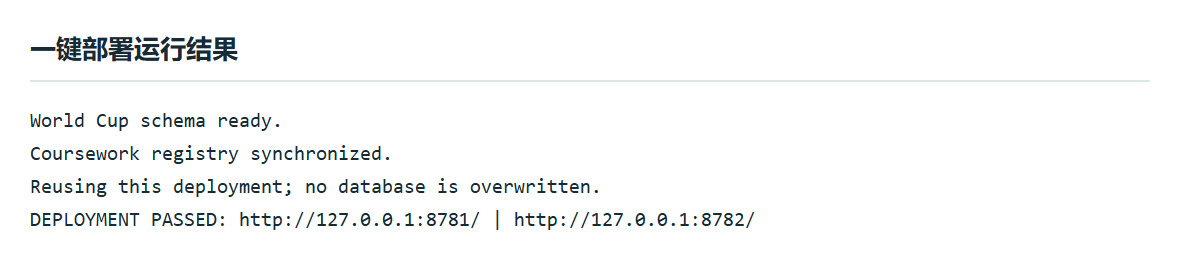
\includegraphics[width=\linewidth,height=.23\textheight,keepaspectratio]{../../figures/14_deployment.png}
\caption{一键部署运行结果}
\end{figure}

\section{再次运行与停止}
再次双击部署脚本，保留数据库和本机配置，更新源码与下载登记，重新检查页面。已有数据不被示例初始化覆盖。端口冲突或未完成的初始化会停止并提示。

使用“停止运行.cmd”关闭本项目记录的PHP进程，再正常关闭独立MySQL；数据保留。再次运行一键部署可恢复服务。修改PHP目录或更换电脑时按环境参数重新定位，不使用原电脑口令。

\section{新库还原与结构更新}
data/install.sql由数据库结构导出，包含20张表及外键、唯一键和COMMENT。还原到专用空数据库后，使用yii worldcup-setup/seed初始化公共样例；账号文件路径由\path{WORLD_CUP_ACCOUNT_FILE}提供。禁止与Yii默认user建表迁移重复执行。后续表结构变化由两人统一维护迁移和字典，并再次导出SQL。

现有文件也可通过scripts/setup.py配置独立空库，接收PHP目录、DSN和用户名，口令交互输入或由一键部署通过标准输入传递。本机配置放.local及main-local.php，不提交Git。

\section{下载与异常处理}
将团队PDF、PPTX和视频放入data/team，个人报告或ZIP放入data/personal，执行yii worldcup-setup/sync-downloads更新登记与摘要。本机保留原个人完整ZIP；公开仓库提供个人报告和项目源码。

数据库连接失败时检查端口、实例日志和权限；缺少扩展时检查php.ini。Composer网络等待时使用本机代理配置，不关闭TLS校验。下载不可用时检查文件路径和摘要后重新登记。PHP内置服务器用于本机课程开发演示，公网部署需配置正式Web服务器和HTTPS。

\end{document}
